\section{Universality} \label{sec:universality}

The search for universal properties, i.e. those that are insensitive to the microscopic details of matter, is an old one. At the atomic level the world is spectacularly complex, with an enormous number of constituent particles interacting with one another in ways that are chaotic and poorly understood. Yet, by the time we reach the macroscopic scale, most of these complexities have been averaged away, and a familiar world emerges. One of the remarkable aspects of this averaging is that different microscopic systems converge to the same macroscopic behaviour. For example, despite enormous variation in chemical composition, all liquids have similar bulk properties, and follow almost identical equations of motion, \textit{more is the same}.% \cite{anderson_more_1972}. 

One of the great successes in understanding this universality was developed in the mid 20th century, starting with the work of Ginzburg and Landau \cite{ginzburg_theory_1950}, and then further developed by a generation of physicists, most notably Ken Wilson \cite{wilson_renormalization_1975} who introduced the concept of the renormalisation group (RG). Let us briefly sketch the central idea using the Ising model as an example, although a thorough discussion is beyond the scope of this thesis, and can be found in Refs.~\cite{cardy_scaling_1996,chaikin_principles_1995}. 

We start with a set of classical spin $\{s_i\}$ arranged on a lattice, interacting according to a general Hamiltonian, for example the Ising Hamiltonian,
\begin{align}
    H = -B \sum_{j} s_j - J \sum_{\braket{jk}} s_j s_k.
\end{align}
Rather than working with individual spins, which can only take two values $\pm 1$, Ginzburg and Landau suggested constructing a smoothly varying local order parameter $m(\textbf x)$ by dividing up these spins into blocks and averaging over each block as seen in Fig.~\ref{fig:rg_flow}a. In this language, the partition function for the model can be rewritten in terms of a path integral over this order parameter
\begin{align}
    \mathcal Z = \sum_{\{s_i\}} e^{-\beta E(s_i)} 
    \rightarrow 
    \int \mathcal D m \sum_{\{s_i\}|m(\textbf x)} e^{-\beta E(s_i)}.
\end{align}
The sum on the right-hand side is arbitrarily difficult, however -- as with tight binding a few decades earlier -- the key insight was that we didn't have to evaluate it at all, rather we could just wrap the quantity up as some unknown free energy
\begin{align}
    \sum_{\{s_i\}|m(\textbf x)} e^{-\beta E(s_i)} = e^{- \beta F(m)},
\end{align}
and make a guess as to the form of the free energy by considering only coefficients that are consistent with the symmetries of the system, for example in an Ising model with no external field, the system has spin-flip symmetry -- so odd powers of $m$ are forbidden,
\begin{align}
    F(m) = \int d^dx 
    \left [ 
    \gamma (\nabla m)^2 
    + \alpha_2 m^2 +  \alpha_4 m^4 + ...
    \right ].
\end{align}
Thus, we have parametrised every possible effective theory for our model with a (possibly infinite) set of prefactors, $\{\gamma, \alpha_n\}$. The next insight came by considering how an effective theory might change under a \textit{rescaling transformation}. There are many ways that this transformation may be formulated, for example one might consider a real-space method, where $m(\textbf x)$ is redefined by choosing some larger block size and averaging $m(\textbf x)$ over this area, effectively zooming out and setting a limit to how finely-resolved the fluctuations in the model can be, shown in Fig.~\ref{fig:rg_flow}b. Equivalently, one can consider imposing a momentum cut-off in the partition function, and integrating out the high momentum modes that correspond to the unwanted small-scale fluctuations. Parametrising this scaling with $\tau$, we find that the coefficients of the free energy pick up a $\tau$-dependence and the rescaling process generates a flow in parameter space $\{\gamma, \alpha_n\} \rightarrow \{\gamma(\tau), \alpha_n(\tau)\}$.
\begin{figure}
    \centering
    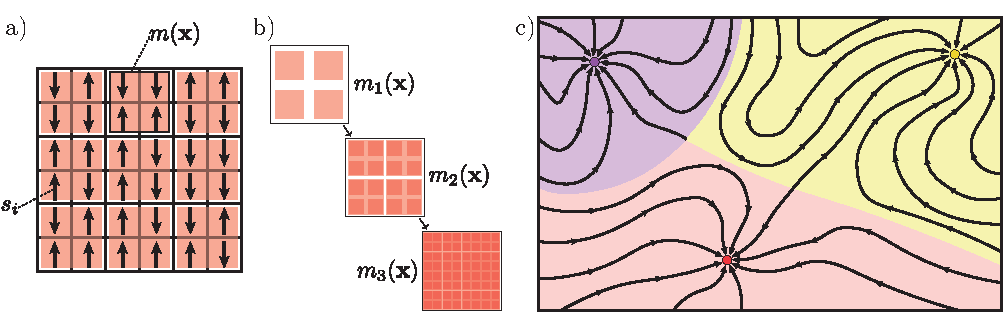
\includegraphics{introduction/figures/rg_flow.pdf}
    \caption[Illustration of a spin-averaging procedure and real space renormalisation step. Diagram of theory space, with a set of stable fixed points.]{
    \textbf{(a)}~In the first step of coarse graining, an averaged magnetisation parameter $m(\textbf x)$ is constructed by choosing and averaging over set of spins $s_i$, each set is indicated with a red box.
    \textbf{(b)}~A real space rescaling can be performed by averaging over successively larger chunks of spins, leading to a set of successively more coarse-grained order parameters $m_i(\textbf x)$. 
    \textbf{(c)}~A heuristic diagram of a parameter space for $F(m)$, where arrows indicate the flow under RG. In each region, the theory flows to one corresponding fixed point, indicated with a circle, which defines the long-range properties of the model. 
    } 
    \label{fig:rg_flow}
\end{figure}

Under this transformation, the points where the free energy functional is static correspond to fixed points where the effective theory becomes scale-invariant, since any dependence on scale implies that the model will change under $\tau$. Remarkably, for many models of interest there turns out to be only a finite number of these fixed points. Under RG flow many microscopically different systems, which start from different points in parameter space, flow to the same fixed point and thus have the same long-range properties, a diagram is shown in Fig.~\ref{fig:rg_flow}c. Thus, the whole of parameter space can be divided into a set of regions, where starting at any point in that region will always flow to the same fixed point, and thus have the same long-range effective description. Thus, any microscopic change to the model, provided that the change does not alter the symmetries of the model, will only have the effect of perturbing the starting point in RG. If this perturbation doesn't move us out of one region and into another, we have the guarantee that the long-range properties of the system are unaffected.

\subsection{The Integer Quantum Hall Effect and Chern Number} \label{sec:qhe}

\begin{figure}
    \centering
    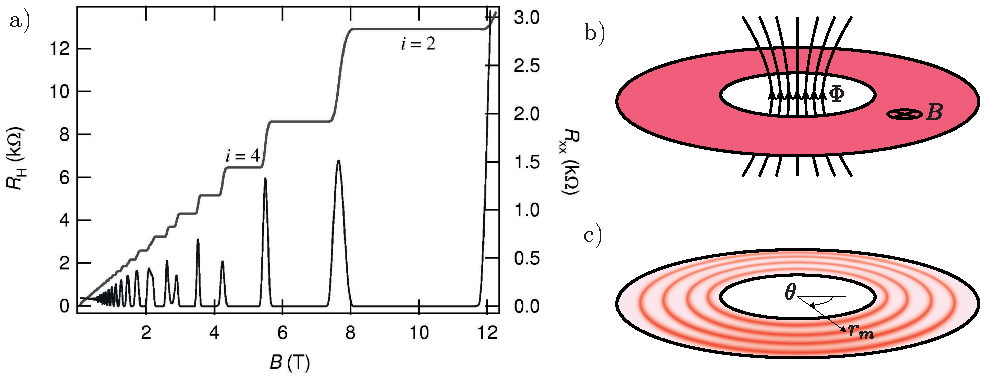
\includegraphics{introduction/figures/QHE.pdf}
    \caption[Hall conductivity as a function of applied magnetic field. A Corbino disc geometry with a sketch of successive states within a Landau level.]{ 
        \textbf{(a)}~The measured resistivity in a GaAs heterostructure at $0.1$ K. \textit{Figure reproduced from \cite{jeckelmann_quantum_2003}.}
        \textbf{(b)}~The geometry proposed by Halperin \cite{haplerin_quantized_1982}. Here a 2D electron gas is confined to the ring, pierced by a transverse magnetic field parametrised by $B$. A flux given by $\Phi$ is threaded through the centre of the ring, which adiabatically increased from $\Phi = 0 \rightarrow \Phi_0$.
        \textbf{(c)}~Depiction of a set of wavefunctions that form part of the lowest Landau level. The $m^{\textup{th}}$ wavefunction is localised to a ring with radius $r_m$. 
    } 
    \label{fig:hall_conductivity}
\end{figure}

In the early 1980s a very different form of universal physics was emerging at the National Laboratory for Intense Magnetic Fields in Grenoble. Here, Klaus von Klitzing was studying the transverse Hall conductivity in silicon-based MOSFETs (metal-oxide-semiconductor field-effect transistor) prepared by Gerhard Dorda and Michael Pepper. These transistors allowed von Klitzing to prepare electrons in a nearly ideal 2D gas at extremely low temperatures and under high magnetic fields. Here, rather than finding the linear relationship between transverse resistivity and applied field predicted by classical Drude theory, von Klitzing found that the transverse resistivity contained a set of plateaux at precisely quantised values given by
\begin{align} \label{eqn:hall_conductivity}
    \rho_{xy} = \frac{2\pi \hbar}{e^2 \nu}, \ \nu\in \mathbb Z,
\end{align}
as shown in Fig.~\ref{fig:hall_conductivity}a \cite{klitzing_new_1980,klitzing_quantizes_1986}. This quantisation was extremely precise, accurate to one part in $10^6$ and has since been adopted as the standard for defining the unit of resistance ($\Omega$) \cite{jeckelmann_quantum_2003}. The precision is particularly surprising given that the samples von Klitzing was using contained fairly substantial disorder. In fact, as we shall see in the following discussion, the presence of some disorder is necessary for producing the sharp jumps in conductivity seen here. 

One of the first steps towards understanding the precise quantisation of the Hall conductivity was proposd by Laughlin \cite{laughlin_quantized_1981}, and developed by Halperin \cite{haplerin_quantized_1982} who considered a quantum Hall system constructed on a ring geometry as shown in Fig.~\ref{fig:hall_conductivity}b. The Hall conductivity could be tested by adiabatically threading some quantity of flux $\Phi$ through the centre of the ring. Including the perpendicular magnetic field and working in symmetric gauge, the electrons experience a magnetic vector potential of the following form,
\begin{align}
    \textbf A = \left ( 
        \frac{1}{2} B r - \frac{\Phi}{2\pi r}    
     \right ) \hat{\bm \theta}.
\end{align}
After solving the Schr\"odinger equation for this potential, one finds the electrons organised into Landau levels (LLs) with energy determined by the cyclotron frequency, $E = \hbar \omega_c(\nu + 1/2)$. The lowest LL consists of a degenerate set of ring-like wavefunctions,
\begin{align}
    \psi_{LLL,m} \sim e^{im\theta} f(r - r_m),
\end{align}
shown in Fig.~\ref{fig:hall_conductivity}c. Here $f(r - r_m)$ is a Gaussian profile, such that the $m^{\textup{th}}$ state is localised to a ring whose radius is determined by the flux enclosed, according to 
\begin{align}
    B\pi r_m^2 = m \Phi_0 + \Phi,
\end{align}
where $\Phi_0 = 2 \pi \hbar / e$ is a single flux quantum. Thus, by adiabatically threading a single flux quantum through the ring (by slowly tuning $\Phi$ from $0 \rightarrow \Phi_0$), we have the effect of transforming each $r_m \rightarrow r_{m+1}$. Each state in the Landau level moves outwards, taking the place of its neighbour, a process known as \textit{spectral flow}. Once the process is complete, the system must be identical to before -- since a whole flux quantum can always be removed with a gauge transformation -- however now there is an extra electron on the outer edge and a missing electron on the inner edge. Thus, the ring behaves like a conveyor belt under flux insertion, transferring a single electron from the inside to the outside, as shown in Fig.~\ref{fig:hall_conductivity_disorder}c. To calculate the resistivity associated with this process, let us suppose the adiabatic process happened over some timescale $T$, and calculate the EMF,
\begin{align}
    \mathcal E = -\frac{\partial \Phi}{\partial t} = -\frac{\Phi_0}{T},
\end{align} 
and the current induced by the transfer of one electron,
\begin{align}
    I = -\frac e T,
\end{align}
giving an overall transverse resistivity of
\begin{align}
    \rho_{xy} = \frac{\mathcal E}{I} = \frac{\Phi_0}{e} = \frac{2\pi \hbar}{e^2}.
\end{align} 
This calculation was performed for a single Landau level; however, the story is straightforwardly transferable to the case when several Landau levels sit below the Fermi energy, since each level independently transports an electron from the inside to the outside edge. Thus, for $\nu$ Landau levels below the Fermi energy, we find an overall conductivity given by Eqn.~\ref{eqn:hall_conductivity}.

\begin{figure}
    \centering
    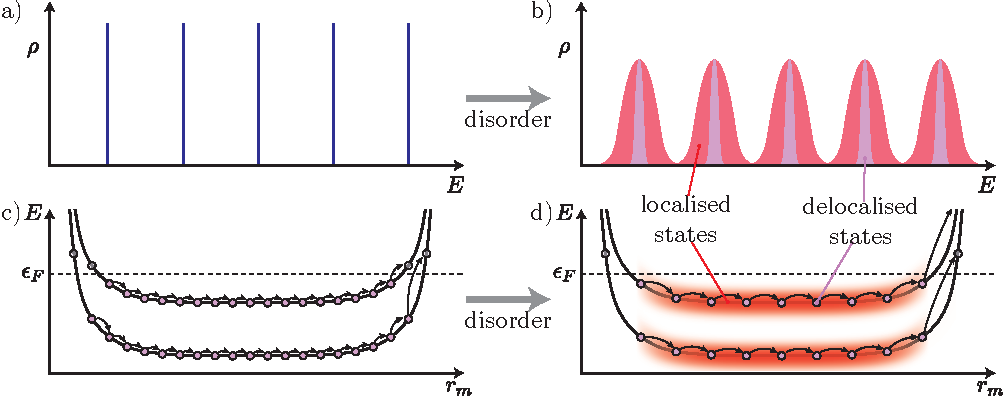
\includegraphics{introduction/figures/QHE_2.pdf}
    \caption[Density of states and energy of landau levels for both a clean and disordered quantum Hall sample on a ring geometry.]{
        \textbf{(a)}~Density of states for a set of five Landau levels in a clean system. Here all states in each LL are degenerate and delocalised around the ring. 
        \textbf{(b)}~In a disordered system, the Landau levels are broadened, and many states become localised. However, each LL still contains a central set of delocalised states.
        \textbf{(c)}~Energy of a set of two Landau levels as a function of radius, showing the effect of a confining potential which raises the energy of Landau levels close to the boundaries. The effect of flux insertion for a clean material on a ring geometry. Here, each Landau level consists of a large number of delocalised states, denoted by the lilac circles. Under flux insertion, each of these states is transported over to the next state, such that by the end of the process each band has a hole on the inner edge, and an excited state on the outer edge.
        \textbf{(d)}~In the disordered case the most of the states in each Landau level have become localised, however a minority of these states remain delocalised. These delocalised states transport an electron across the ring for the same reason as in the clean material. 
    } 
    \label{fig:hall_conductivity_disorder}
\end{figure}

Let us now consider adding a disorder potential $V(\textbf r)$ to the system. To preserve the Hall effect, one must assume that this disorder is not strong enough to mix different Landau levels, $|V| < \hbar \omega_c$. Adding such a term will break the degeneracy within each Landau level, leading to a smearing out of the density of states into broad peaks. In addition, while the clean Landau levels are composed of delocalised states, in the disordered bands most of the states will become localised. However, in the centre of each band, there will remain a minority of delocalised states, as shown in Fig.~\ref{fig:hall_conductivity_disorder}b. \todo{Perhaps say something about where these localised states come from! i.e. Chalker Coddington and the percolation picture...}

The localised states are no longer able to change under flux insertion, since the effect of the threaded flux on a state that does not wrap the whole ring can always be removed with a gauge transformation. The remaining delocalised states will still be able to see the flux insertion, and so will still undergo spectral flow. As before, each delocalised state is adiabatically transformed onto the next delocalised state away from the centre of the ring, as shown in Fig.~\ref{fig:hall_conductivity_disorder}d. Thus, provided that some states remain delocalised, the net effect is still to transport a single electron from the inside to the outside of the ring. In fact, it was shown by Prange \cite{prange_quantized_1981} that when a single state is localised, the nearby delocalised states will `speed up' to compensate for the missing current from the localised state. Thus, we see that as disorder is increased, the quantised Hall conductance remains, transported by a shrinking minority of delocalised states in each Landau level.

It is precisely the fact that a small minority of states are responsible for the Hall conductivity that stabilises the plateaux shown in Fig.~\ref{fig:hall_conductivity}a. Here, the tuning of the applied field $B$ has the effect of shifting the energy and degeneracy of the Landau levels -- effectively sweeping the Fermi level across the LL spectrum. The conductivity is determined only by the number of filled LLs, however only the extended states in the centre are able to transport charge. Thus, the conductivity is only allowed to change at the point where the Fermi energy sweeps through these states. The stronger the disorder (within reason), the fewer delocalised states are present which means that the transition between plateaux becomes sharper and the plateaux themselves are more precisely quantised. 

The Laughlin/Halperin picture was one of the first -- and simplest -- explanations for the quantised Hall conductivity and its remarkable insensitivity to disorder. However, in the following years a much deeper mathematical picture was uncovered, starting with the work of Thouless and his collaborators \cite{thouless_quantized_1982}, who calculated the transverse conductivity using the Kubo formula~\cite{kubo_statistical-mechanical_1957}. Working in periodic boundaries, they showed that the conductivity may be constructed as a Brillouin-zone integral that evaluated the phase change of the Bloch eigenstate around the unit cell. Because the state must remain single-valued over $\textbf k$, this integral was necessarily quantised to multiples of $2\pi$, and thus the conductivity had to be quantised on any periodic system. Independently, Michael Berry was considering the adiabatic theorem, \cite{berry_quantal_1984} and showed that when a quantum system was transformed adiabatically around a closed loop in parameter space the final state would pick up some extra phase, now called Berry's phase, which could be interpreted as a surface integral. Although it was not immediately obvious to Berry or Thouless,\footnote{Reportedly Berry contacted David Thouless to ask if he thought these phases had anything to do with his TKNN invariant and Thouless responded that it was doubtful there was any connection \cite{simon_berrys_2020}.} Avron, Seiler and Simon showed that these ideas were profoundly linked, both deriving from the same concepts in differential geometry \cite{avron_homotopy_1983,simon_holonomy_1983}. Berry's phase was really the geometric angle accumulated by parallel transport around a closed path -- the holonomy -- which could be re-expressed as an integral of the curvature over the surface enclosed. Similarly, the TKNN invariant was actually a topological invariant -- the first Chern number, $\mathcal Q$ -- of the mapping from the Brillouin zone to the Hilbert space, found by integrating Berry's curvature over the entire Brillouin zone. \todo{Stick equation in here} A detailed explanation of the Chern invariant is given in Chapter \ref{chap:chern_intro}. 
\begin{figure}
    \centering
    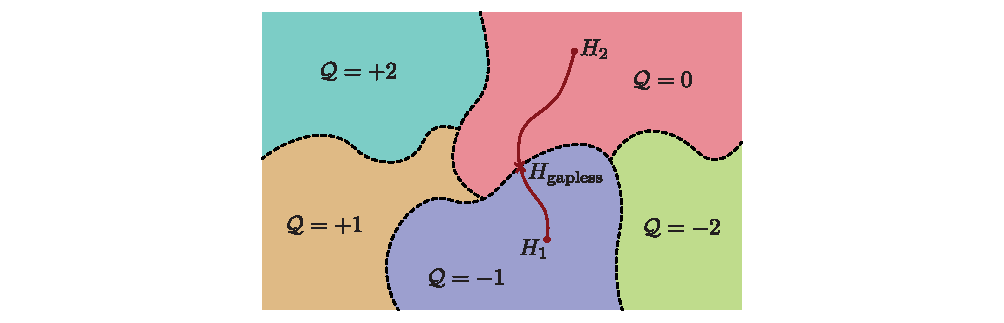
\includegraphics{introduction/figures/chern_classes.pdf}
    \caption[Illustration of the space of all non-interacting Hamiltonians, classified by their Chern numbers.]{
        The space of all Hamiltonians can be divided into a set of Chern classes defined by the bands' Chern numbers (only one band's Chern number is shown in this illustration). Adiabatically transforming from one Hamiltonian $H_1$ to another $H_2$ in a different Chern class, one necessarily crosses a point where the Hamiltonian becomes gapless.
    } 
    \label{fig:chern_classes}
\end{figure}

Using these methods, it was now possible to associate a quantised Chern number to each energy level in the band structure of a material. As per the original motivation, the Chern number determined the contribution of each band to the Hall conductivity. However, one could also view these invariants as a remarkably universal framework for classifying Hamiltonians, since their quantised nature meant that a band's Chern number could not change under adiabatic deformation of the system without closing the band gap (at which point the band, and thus $Q$, would be ill-defined). Thus, two Hamiltonians with different Chern numbers sit in two different Chern classes, where it is not possible to deform one into the other without a gap closing. Of course, these invariants strictly only applied to systems with a notion of band structure, i.e.~for non-interacting systems with translational symmetry. Several proposals exist for extending these invariants to interacting or disordered materials, most notably the construction of a local Chern marker \cite{kitaev_anyons_2006, markov_local_2021, loring_guide_2019, bianco_mapping_2011} which we shall discuss in Chapter \ref{chap:local_markers}. The simplest extension can be found by noting that the topological class of a Hamiltonian can only change with a closing of the band gap. Thus, as long as a general quantum system has a gapped ground state, and can (without closing this gap) be adiabatically connected to a Hamiltonian with well-defined Chern number, then the two systems are considered to have the same Chern numbers \cite{varney_topological_2011}. Thus, we see that, in analogy with the case of RG and universality discussed in the previous section, the Chern classification describes a set of physical properties that are deeply ambivalent to the microscopics of a model. Any changes to the system that do not close the band gap will have no effect on the Chern class or the Hall conductivity.
